% ====================================================================
% §4 히스테리시스 분기 중심 (N3)
% ====================================================================
\section{히스테리시스 분기 중심 (N3)}\label{sec:hys}
평형 중심 $U_j$ 는 상호작용 $\Omega_j$ 와 분기 인자 $\gamma_j$ 가 있으면 방향별 분기 중심 $U_j^{\,d}$ 로 이동한다
(그렇지 않으면 $U_j$ 그대로). 본 문건의 주 전개는 방전이며, 히스테리시스는 그 위의 \emph{구조적 분기}로 선언된다 --- 방전과 충전이
같은 전이를 서로 다른 준안정 가지로 과주행해 중심이 갈라진다(삽입형 전극 히스테리시스의 열역학적 기원\cite{dreyer2010}).
이 절은 그 gap 의 닫힌 식과 부호를, 격자기체 자유에너지의
이중웰에서 spinodal 을 거쳐 단계적으로 유도한다.

유도에 들어가기 전에 이 분기의 물리적 계보와 두 용어를 놓는다. 상분리 삽입 전극에서는 충$\cdot$방전
전위의 갈림이 전류를 $0$ 으로 줄여도 사라지지 않음이 실측된다 --- 서론의 관측이 말한 잔존 성분이며, 그
기원이 저항$\cdot$분극 같은 동역학이 아니라 \emph{비단조 자유에너지를 갖는 계의 준안정성}이라는 것이
Dreyer 등의 열역학 분석이다\cite{dreyer2010,dreyer2011}. \emph{준안정 가지}(metastable branch)는
국소적으로는 안정하나 전역 최소는 아닌 상태들의 연속이고, \emph{과주행}(overshoot)은 진행이 평형
전환점(Maxwell 전위)을 지나서도 그 가지를 따라 더 나아가는 것이다 --- 이상 단일 입자가 과주행할 수 있는
상한이 spinodal(자유에너지 곡률이 $0$ 이 되는 안정성 한계)이며, 이 절의 gap 닫힌 식이 바로 그 상한이다.
$N$ 개 입자 앙상블이 같은 그림 위에서 평탄역을 만드는 경로는 \S\ref{sec:broadening}(iii-a)가 잇는다.

\subsection{상호작용이 평형을 비트는 곳 --- $\mu(\theta)$ 의 상호작용 몫}\label{sec:hys-spinodal}
\textbf{(a) 출발 --- Part 0 의 결과 받기.} 한 전이를 ``동등한 자리에 리튬이 차고 비는'' 격자기체로 보면,
점유율 $\theta$ 의 화학퍼텐셜과 진행률 좌표의 정규용액 자유에너지는 Part 0 이 세운
식~\eqref{eq:mu}$\cdot$\eqref{eq:gxi} 그대로다($\Omega_j>0$ 이면 동종 이웃 인력 --- 가운데를 위로 밀어
이중웰의 씨앗, 식~\eqref{eq:sm-thresh}). \textbf{(b) 연산 --- 두 번 미분.}
식~\eqref{eq:gxi} 를 두 번 $\xi$ 로 미분하면(로그 몫의 1계 미분 $RT\ln[\xi/(1-\xi)]$, 2계 미분
$RT/[\xi(1-\xi)]$; 상호작용 몫의 2계 미분 $-2\Omega$)
\begin{equation}
g_j''(\xi)=\frac{RT}{\xi(1-\xi)}-2\Omega_j.
\label{eq:gpp}
\end{equation}
\textbf{(c) spinodal --- $g_j''=0$ 의 근.} $g_j''=0$ 은 $\xi(1-\xi)=RT/(2\Omega_j)$, 곧 $\xi^2-\xi+RT/(2\Omega_j)=0$
의 근의 공식으로
\begin{equation}
\xi_{s,j}^\pm=\tfrac12(1\pm u_j),\qquad
u_j\equiv\sqrt{1-\frac{2RT}{\Omega_j}}\quad(\Omega_j>2RT).
\label{eq:spinodal}
\end{equation}
$u_j$ 가 실수가 되는 조건 $\Omega_j>2RT$ 가 상분리(따라서 히스테리시스)의 문턱이며($g''<0$ 구간이 생겨 한 전위에 여러
$\xi$ --- 그림~\ref{fig:doublewell}), $\Omega_j\le2RT$ 면 갈라짐이 없다. 이 문턱을 넘지 못하면($\Omega_j\le2RT$) 분기 gap 은 정확히 0 이다(식~\eqref{eq:dUhys} 참조).

\begin{figure}[t]
\centering
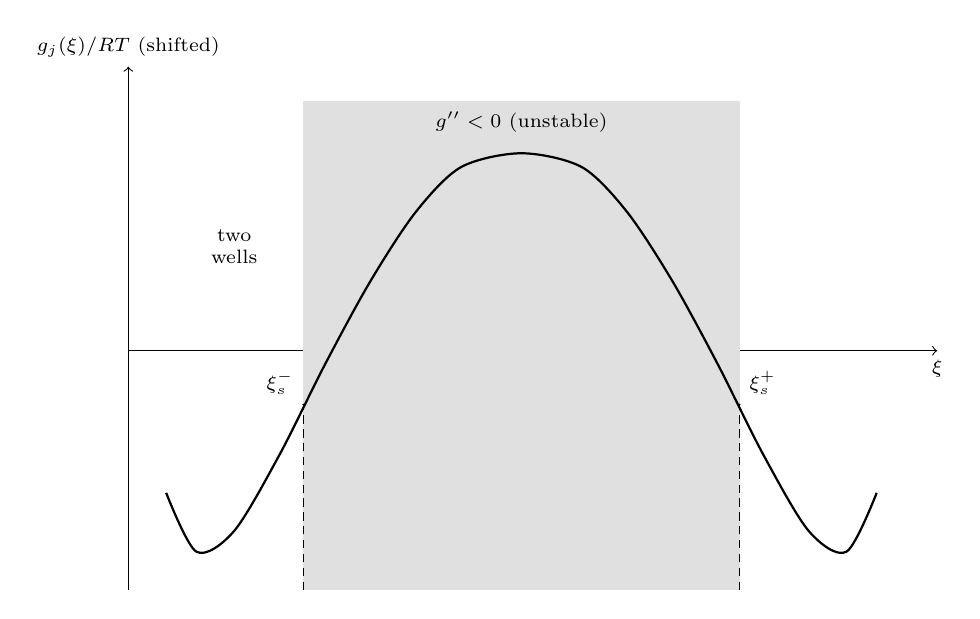
\begin{tikzpicture}[x=9.6cm,y=44cm]
% double-well free energy g(xi) for Omega=3RT (qualitative shape, normalized)
\draw[->] (-0.02,-0.069) -- (-0.02,0.082) node[above,font=\scriptsize] {$g_j(\xi)/RT$ (shifted)};
\draw[->] (-0.02,0) -- (1.05,0) node[below,font=\scriptsize] {$\xi$};
\foreach \xx in {0.25,0.5,0.75} {\draw (\xx,0.0015) -- (\xx,-0.0015) node[below,font=\scriptsize] {\xx};}
% spinodal band (g''<0) shading
\fill[black!12] (0.2113,-0.069) rectangle (0.7887,0.072);
\node[font=\scriptsize] at (0.5,0.066) {$g''<0$ (unstable)};
% the double well curve
\draw[thick] plot[smooth] coordinates {(0.03,-0.041) (0.07,-0.058) (0.12,-0.052) (0.18,-0.030) (0.24,-0.004) (0.3,0.020) (0.36,0.040) (0.42,0.053) (0.5,0.057) (0.58,0.053) (0.64,0.040) (0.7,0.020) (0.76,-0.004) (0.82,-0.030) (0.88,-0.052) (0.93,-0.058) (0.97,-0.041)};
% spinodal points
\fill (0.2113,-0.0155) circle (0.35pt) node[above left,font=\scriptsize] {$\xi_s^-$};
\fill (0.7887,-0.0155) circle (0.35pt) node[above right,font=\scriptsize] {$\xi_s^+$};
\draw[densely dashed] (0.2113,-0.069) -- (0.2113,-0.0155);
\draw[densely dashed] (0.7887,-0.069) -- (0.7887,-0.0155);
\node[font=\scriptsize,align=center] at (0.12,0.030) {two\\wells};
\end{tikzpicture}
\caption{격자기체 자유에너지 $g_j(\xi)$ (식~\eqref{eq:gxi} 의 \emph{개형}, $\Omega_j=3RT$ --- 정성 곡선;
수치 정확 좌표는 그림~\ref{fig:sm-gxi} 의 같은 곡선). $\Omega>2RT$ 면 가운데가
언덕이 되어 양쪽에 골짜기 둘 --- 음영 띠($g''<0$, 식~\eqref{eq:gpp})가 변곡점 $\xi_s^\pm$ (spinodal, 식~\eqref{eq:spinodal})
사이의 불안정 구간이다. 이 곡률 부호 전환이 \S\ref{sec:hys} 의 비단조 전위 곡선과 분기 gap 을 낳는다.}
\label{fig:doublewell}
\end{figure}

\subsection{gap 의 닫힌 꼴 --- 두 spinodal 의 전위 차}\label{sec:hys-gap}
\textbf{(a) 출발 --- 비단조 평형 전위 곡선.} 평형 조건~\eqref{eq:eqcond}($\mu=\mu^0-sF(V-U)$, 배치 몫 자유에너지 기울기 $=$ 전기화학 구동력)에 의해 자유에너지~\eqref{eq:gxi} 의 1계 미분이 곧 평형 전위에 묶인다
($g_j'(\xi)=RT\ln[\xi/(1-\xi)]+\Omega_j(1-2\xi)=sF(V_\eq-U_j)$). 1차(직선) 몫을 뗀 식~\eqref{eq:gxi} 가 \emph{1계} 미분에서도
옳은 근거는 Part 0 이 세운 조성 몫의 우함수 대칭(\S\ref{sec:sm-mf}: $f(1-\xi)=f(\xi)$, 따라서 $f'(1-\xi)=-f'(\xi)$)이다
--- 식~\eqref{eq:mu} 의 $\mu_\mathrm{Li}(\theta)-\mu^0=f'(\theta)$
에 $\theta=1-\xi$ 를 넣으면 $\mu_\mathrm{Li}-\mu^0=f'(1-\xi)=-f'(\xi)=-g_j'(\xi)$ 가 되고, 뗀 선형 몫이 남긴 상수 $\mu^0$ 가
식~\eqref{eq:eqcond} 양변에서 상쇄돼 선형항 없이도 위 등식이 성립한다. 이를 $V_\eq$ 로 풀면
\begin{equation}
V_{\eq,j}(\xi)\;=\;U_j+\frac{RT}{sF}\ln\frac{\xi}{1-\xi}+\frac{\Omega_j}{sF}\,(1-2\xi),
\label{eq:Veq}
\end{equation}
이고 $\Omega_j>2RT$ 면 비단조다 --- 방전은 $\xi\!\approx\!0$ 에서 상승 가지를 극대 $\xi_{s,j}^-$ 까지, 충전은 $\xi\!\approx\!1$
에서 극소 $\xi_{s,j}^+$ 까지 과주행하므로(전위 곡선의 극값이 $\dd V_\eq/\dd\xi=g_j''/sF=0$, 곧 spinodal 과 같은 점 ---
그림~\ref{fig:hysloop}), 두 극값의 전위 차가 분기 gap 의 spinodal 상한이다. \textbf{(b) 연산 --- spinodal 값 대입.}
식~\eqref{eq:spinodal} 의 $\xi_{s,j}^\pm=\tfrac12(1\pm u_j)$ 를 식~\eqref{eq:Veq} 의 두 비상수 항에 넣으면, logit 인자와
$(1-2\xi)$ 인자가 두 끝점에서 각각
\begin{equation}
\frac{\xi}{1-\xi}\bigg|_{\xi_{s,j}^\pm}=\frac{1\pm u_j}{1\mp u_j},
\qquad
(1-2\xi)\big|_{\xi_{s,j}^\pm}=\mp u_j
\label{eq:hyssub}
\end{equation}
--- 곧 두 끝점에서 logit 인자가 서로 역수다. \textbf{(c) 중간식 --- 극대에서 극소 빼기.} 극값 차를 적으면 상수항 $U_j$ 가
상쇄되고
\begin{align}
\Delta U_j^\hys
&=V_{\eq,j}(\xi_{s,j}^-)-V_{\eq,j}(\xi_{s,j}^+)\notag\\
&=\frac{RT}{sF}\Big[\ln\frac{1-u_j}{1+u_j}-\ln\frac{1+u_j}{1-u_j}\Big]
+\frac{\Omega_j}{sF}\big[u_j-(-u_j)\big]\notag\\
&=-\frac{4RT}{sF}\,\mathrm{artanh}\,u_j+\frac{2\Omega_j}{sF}\,u_j
\label{eq:hysdiff}
\end{align}
(둘째 줄의 두 로그가 부호 반대 같은 크기라 $\ln[(1-u)/(1+u)]-\ln[(1+u)/(1-u)]=-2\ln[(1+u)/(1-u)]=-4\,\mathrm{artanh}\,u$,
$\mathrm{artanh}\,u=\tfrac12\ln\tfrac{1+u}{1-u}$ 사용). \textbf{(d) 박스 --- $s=+1$ 정리.}
\begin{equation}
\boxed{\;\Delta U_j^\hys
=\frac{2}{F}\Big[\Omega_j\,u_j-2RT\,\mathrm{artanh}\,u_j\Big],
\qquad u_j=\sqrt{1-\frac{2RT}{\Omega_j}}\;.}
\label{eq:dUhys}
\end{equation}
$\Omega_j\le2RT$ 면 gap 은
정확히 $0$ 이다(제곱근이 허수가 되는 영역의 명시 분기). 부호 --- 극대 $>$ 극소라 $\Delta U_j^\hys\ge0$ 이고, $\Omega_j\to2RT^+$ 에서
$u_j\to0$ 이라 Taylor 전개로 $\Delta U_j^\hys\to\frac{8RT}{3F}u_j^3\to0$ 으로
연속이다($u_j^3\propto(T_{c,j}-T)^{3/2}$, $T_{c,j}=\Omega_j/2R$ --- 임계온도에서 매끄럽게 소멸). \textbf{★Taylor 전개의 함정
--- 두 급수를 함께 전개해야 한다.} 위 $\frac{8RT}{3F}u^3$ 극한은 식~\eqref{eq:dUhys} 의 두 항 $\Omega_ju_j$ 와
$2RT\,\mathrm{artanh}\,u_j$ 를 \emph{함께} $u\to0$ 으로 전개해야 얻어진다. $u_j$ 정의를 뒤집으면
$\Omega_j=2RT/(1-u_j^2)$ 이라 $\Omega_ju_j=2RT(u_j+u_j^3+\cdots)$ 이고, 다른 항은 $\mathrm{artanh}\,u=u+u^3/3+\cdots$ 이므로
$\frac{2}{F}[\Omega_ju-2RT\,\mathrm{artanh}\,u]=\frac{2}{F}[2RT(u+u^3)-2RT(u+u^3/3)]=\frac{8RT}{3F}u^3$ 로 \emph{양수}로 소멸한다.
반면 $\Omega_j\approx2RT$ 를 첫째 항에 \emph{상수 대입}만 하고 $\mathrm{artanh}$ 만 전개하면
$\frac{2}{F}[2RT\cdot u-2RT(u+u^3/3)]=-\frac{4RT}{3F}u^3$ 로 \emph{부호가 뒤집힌} 오답에 이른다 --- $\Omega_j$ 가
$u_j$ 를 통해 $u^3$ 차수에 기여하는 몫을 빠뜨렸기 때문이다. 곧 임계온도 근방의 gap 은 반드시 양수로 소멸하며,
상수 대입은 물리적으로 무의미한 음의 gap 을 준다. 문턱·양수 연성 개시·상수-대입 오답·임계 소멸의 네 논점은
그림~\ref{fig:hysgap} 이 정확식의 수치 평가로 한 장에 모은다.

\begin{figure}[t]
\centering
\resizebox{\textwidth}{!}{%
\begin{tikzpicture}[>=Latex]
% =============== (a) 무차원 gap vs Omega/RT ===============
\begin{scope}[x=1.02cm,y=0.72cm]
% threshold band (single phase, gap identically 0)
\begin{scope}[on background layer]
  \fill[black!6] (0,-0.62) rectangle (2,5.62);
\end{scope}
\draw[->] (0,0) -- (6.55,0) node[right,font=\scriptsize] {$\Omega_j/RT$};
\draw[->] (0,-0.62) -- (0,5.62) node[above,font=\scriptsize] {$F\,\Delta U_j^\hys/RT$};
\foreach \xx in {1,2,3,4,5,6} {\draw (\xx,0.05) -- (\xx,-0.05) node[below,font=\scriptsize] {\xx};}
\foreach \yy in {1,2,3,4,5} {\draw (0.05,\yy) -- (-0.05,\yy) node[left,font=\scriptsize] {\yy};}
% threshold marker
\draw[densely dotted] (2,-0.62) -- (2,5.62);
\node[font=\scriptsize,align=center] at (1.0,3.1) {$\Omega_j\le2RT$:\\gap $\equiv0$\\(단상)};
% exact closed form (eq:dUhys), dimensionless
\draw[very thick] (0,0) -- (2,0);
\draw[very thick] plot[smooth] coordinates {(2,0) (2.02,0.0027) (2.05,0.0105) (2.1,0.0294)
  (2.2,0.0819) (2.35,0.1858) (2.5,0.3112) (2.75,0.5547) (3,0.8302) (3.25,1.13) (3.5,1.449)
  (3.75,1.7836) (4,2.1314) (4.5,2.8585) (5,3.6191) (5.5,4.4057) (6,5.2131)};
\node[font=\scriptsize,rotate=40] at (5.05,4.05) {정확식~\eqref{eq:dUhys}};
% soft cubic onset (8/3)u^3
\draw[densely dotted,thick] plot[smooth] coordinates {(2,0) (2.02,0.0026) (2.05,0.0102)
  (2.1,0.0277) (2.2,0.0731) (2.35,0.1533) (2.5,0.2385) (2.75,0.3798) (3,0.5132)
  (3.25,0.6361) (3.5,0.7482)};
\node[font=\scriptsize,anchor=west] at (3.28,0.42) {$\tfrac83u_j^3$ (연성 개시)};
% wrong constant-substitution Taylor: -(4/3)u^3
\draw[dashed,black!50] plot[smooth] coordinates {(2,0) (2.02,-0.0013) (2.05,-0.0051)
  (2.1,-0.0139) (2.2,-0.0365) (2.35,-0.0766) (2.5,-0.1193) (2.75,-0.1899) (3,-0.2566)
  (3.25,-0.318) (3.5,-0.3741)};
\node[font=\scriptsize,black!50,anchor=west] at (2.42,-0.95) {상수 대입 오답 $-\tfrac43u_j^3<0$};
\draw[->,thin,black!50] (3.05,-0.78) -- (3.28,-0.40);
% cross-check markers
\fill (3,0.8302) circle (1.1pt); \fill (4,2.1314) circle (1.1pt);
\node[font=\scriptsize,anchor=south east] at (3.06,0.90) {$(3,\,0.830)$};
\node[font=\scriptsize,anchor=south east] at (4.06,2.20) {$(4,\,2.131)$};
\node[font=\scriptsize] at (3.3,-1.55) {(a) 문턱$\cdot$연성 개시$\cdot$부호 함정};
\end{scope}
% =============== (b) gap(T) [mV], four staging Omega ===============
\begin{scope}[xshift=8.15cm,x=0.01235cm,y=0.0323cm,shift={(-240,0)}]
% operating window 260-340 K
\begin{scope}[on background layer]
  \fill[black!6] (260,0) rectangle (340,130);
\end{scope}
\draw[->] (240,0) -- (815,0) node[right,font=\scriptsize] {$T$ [K]};
\draw[->] (240,0) -- (240,130) node[above,font=\scriptsize] {$\Delta U_j^\hys(T)$ [mV]};
\foreach \xx in {300,400,500,600,700,800} {\draw (\xx,1.5) -- (\xx,-1.5) node[below,font=\scriptsize] {\xx};}
\foreach \yy in {25,50,75,100,125} {\draw (244,\yy) -- (236,\yy) node[left,font=\scriptsize] {\yy};}
\node[font=\tiny,black!55,anchor=north] at (321,127) {측정 창};
% 298.15 K guide
\draw[densely dotted] (298.15,0) -- (298.15,127);
% Omega = 13000 (2->1)
\draw[very thick] plot[smooth] coordinates {(240,125.375) (260,117.298) (280,109.546)
  (300,102.101) (320,94.95) (340,88.078) (360,81.477) (380,75.137) (400,69.049)
  (420,63.208) (440,57.609) (460,52.247) (480,47.118) (500,42.221) (520,37.553)
  (540,33.115) (560,28.906) (580,24.929) (600,21.185) (620,17.68) (640,14.42)
  (660,11.413) (680,8.671) (700,6.21) (720,4.055) (740,2.243) (760,0.84)
  (770,0.333) (777.8,0.066) (781.5,0.001)};
% Omega = 10000 (2L->2)
\draw[thick] plot[smooth] coordinates {(240,75.212) (260,68.272) (280,61.683)
  (300,55.432) (320,49.505) (340,43.894) (360,38.59) (380,33.589) (400,28.887)
  (420,24.483) (440,20.378) (460,16.576) (480,13.083) (500,9.911) (520,7.075)
  (540,4.6) (560,2.528) (580,0.932) (590,0.36) (597.4,0.075) (601.1,0.002)};
% Omega = 8000 (3->2L)
\draw[thick,black!55] plot[smooth] coordinates {(240,44.346) (260,38.459) (280,32.963)
  (300,27.849) (320,23.11) (340,18.743) (360,14.751) (380,11.142) (400,7.929)
  (420,5.137) (440,2.808) (460,1.024) (470,0.389) (477.1,0.084) (480.8,0.002)};
% Omega = 6000 (4->3)
\draw[thick,densely dashed] plot[smooth] coordinates {(240,17.332) (260,13.028)
  (280,9.226) (300,5.947) (320,3.23) (340,1.163) (350,0.433) (356.8,0.097) (360.5,0.002)};
% Tc ticks on axis (labels folded into curve tags below)
\foreach \tc in {360.8,481.1,601.4,781.8} {\draw[black!60,semithick] (\tc,0) -- (\tc,3.4);}
\draw[->,thin,black!60] (742,13.5) -- (778,1.5);
\node[font=\tiny,black!60,anchor=south] at (726,13.2) {눈금 $=T_{c,j}{=}\Omega_j/2R$};
% intersections at 298.15 K
\fill (298.15,102.78) circle (1.1pt) node[right,font=\tiny] {$102.8$};
\fill (298.15,56.00) circle (1.1pt) node[right,font=\tiny] {$56.0$};
\fill (298.15,28.31) circle (1.1pt) node[right,font=\tiny] {$28.3$};
\fill (298.15,6.23) circle (1.1pt) node[above right,font=\tiny] {$6.2$};
% curve labels (with their Tc)
\node[font=\tiny,anchor=west] at (556,32.5) {$\Omega{=}13000$ ($T_c\,782$ K)};
\node[font=\tiny,anchor=west] at (462,20.5) {$10000$ ($601$ K)};
\node[font=\tiny,anchor=west] at (390,14.2) {$8000$ ($481$ K)};
\node[font=\tiny,anchor=west] at (316,6.8) {$6000$ J/mol ($361$ K)};
% closing annotation
\node[font=\scriptsize,align=left,anchor=north west] at (480,122)
  {$T\!\to\!T_c{=}\Omega_j/2R$:\\ gap $\propto(T_c{-}T)^{3/2}$ 소멸\\ (도핑 $\Omega\!\downarrow$ 도 같은 축)};
\node[font=\scriptsize] at (520,-22) {(b) 온도$\cdot$$\Omega$ 에 따른 gap 소멸 (staging 초기값 4건)};
\end{scope}
\end{tikzpicture}%
}
\caption{히스테리시스 gap 닫힌 꼴 $\Delta U_j^\hys$(식~\eqref{eq:dUhys})의 전 거동 --- 좌표는 식
그대로의 수치 평가. (a) 무차원 gap $F\Delta U_j^\hys/RT=2[\omega u_j-2\,\mathrm{artanh}\,u_j]$
($\omega\equiv\Omega_j/RT$, $u_j=\sqrt{1-2/\omega}$): 문턱 $\Omega_j\le2RT$(음영)에서 정확히 $0$,
문턱 직후 두 급수를 함께 전개한 $\tfrac83u_j^3$(점선)으로 \emph{양수} 연성 개시하며, $\Omega_j$ 를
상수 대입만 한 잘못된 전개는 $-\tfrac43u_j^3$(회색 파선)로 부호가 뒤집힌다(본문 ★Taylor 전개의 함정).
점 $(4,\,2.131)$ 은 그림~\ref{fig:hysloop} 의 $\Omega_j{=}4RT$ gap 과 같은 값이다.
(b) 표~\ref{tab:staging} 의 $\Omega_j$ 초기값 4건을 mV 로 평가한 $\Delta U_j^\hys(T)$: 각 곡선은
자기 임계온도 $T_{c,j}=\Omega_j/2R$(축 눈금)에서 $(T_c-T)^{3/2}$ 로 매끄럽게 소멸한다 --- 승온과
도핑에 의한 $\Omega_j$ 감소(식~\eqref{eq:lco-dope})가 같은 축 위에서 gap 을 닫는 두 손잡이다.
점선 수직선은 $298.15$ K, 그 교점 수치는 spinodal 상한 gap 이며 실측 분기는 $\gamma_j$ 배 안쪽이다
(식~\eqref{eq:Ubranch}).}
\label{fig:hysgap}
\end{figure}
% 자산(v1.0.21 신규): [V21-R-02 히스 gap 전 거동 fig:hysgap — FIGS_PICK N-2(베이스 FF1-1)]

\subsection{방향별 분기 중심 $U_j^{\,d}$}\label{sec:hys-branch}
\textbf{(a) 출발 --- 두 spinodal 끝점의 평균.} 식~\eqref{eq:hyssub} 의 두 대입값으로 두 끝점의 \emph{평균}을 적으면
로그 몫 합 $\ln\frac{1-u}{1+u}+\ln\frac{1+u}{1-u}=0$ 과 $(1-2\xi)$ 몫 합 $u+(-u)=0$ 이 둘 다 $0$ 이라
\begin{equation}
\tfrac12\big[V_{\eq,j}(\xi_{s,j}^-)+V_{\eq,j}(\xi_{s,j}^+)\big]=U_j
\label{eq:hyssym}
\end{equation}
--- 분기는 $U_j$ 대칭이다. \textbf{(b)(c) 한 자유도로.} 이 대칭 위에서 실측 분기 중심을 방향별 한 자유도로 적으면(축소
인자 $\gamma_j$ 와 부분 cycle 인자 $h_{\eta,j}$ 를 곱해)
\begin{equation}
\boxed{\;U_j^{\,d}\;=\;U_j\;+\;\tfrac12\,\sigma_d\,h_{\eta,j}\,\gamma_j\,\Delta U_j^\hys\;.}
\label{eq:Ubranch}
\end{equation}
\textbf{(d) 부호.} 방전($\sigma_d=+1$)은 중심을
$+$ 쪽, 충전($\sigma_d=-1$)은 $-$ 쪽으로 옮겨 $U_j^{\dis}>U_j^{\chg}$ --- 탈리튬화 가지가 높은 전위에
남는다는 영전류 극한의 실측 갈림\cite{dreyer2010} 과 부호가 일치한다.
$\gamma_j=1$ 이 spinodal 상한, $\gamma_j\to0$ 이 히스 소멸, $h_{\eta,j}$ 가 부분 cycle 보정(기본 $1$)이다.
두 인자의 지위를 명확히 하면 --- spinodal 상한은 결함$\cdot$요동$\cdot$불균일이 전혀 없는 이상 단일 입자가
안정성 한계까지 버틴다는 극한이고, 실재 전극은 대개 그 전에(국소 요동$\cdot$불균일 핵생성으로) 가지를
이탈하므로 실측 gap 은 상한보다 안쪽에 앉는다 --- 그 축소를 전이당 한 계수로 흡수한 현상학 인자가
$\gamma_j\in[0,1]$ 이다. $h_{\eta,j}$ 는 완전 cycle 을 전제한 분기가 부분 cycle 이력에서 덜 벌어지는 것을
담는 보정 인자다. 두 인자 모두 값은 피팅이 정하며, spinodal gap $\Delta U_j^\hys$ 는 그 피팅값이 넘을 수
없는 열역학 상한을 준다.

전이당 필요한 것은 상수인 분기 shift 뿐이므로, 식~\eqref{eq:Ubranch} 의 $U_j$ 자리에 $0$ 을 대입해 shift
분만 얻고, 배열 중심 $U_j$ 에 더한다:
\begin{equation}
\mathrm{center}=
\begin{cases}
U_j+\tfrac12\sigma_d h_{\eta,j}\gamma_j\Delta U_j^\hys(T_\rep) & \gamma_j\ne0 \text{ 이고 } \Omega_j>0\\[2pt]
U_j & \text{그 외(분기 없음)}.
\end{cases}
\label{eq:center}
\end{equation}
이 분기 중심(식~\eqref{eq:center})이 다음 절 평형 진행률 $\xi_\eq$ 의 중심으로 들어간다. 평형 종의 \emph{모양} 자체는 방향 불변이고,
방향이 바꾸는 것은 이 중심의 위치(와 \S\ref{sec:tail} 의 꼬리 방향)뿐이다.

\begin{figure}[t]
\centering
% T3 fig:hysloop  (quantitative-density)
% Coordinates = exact numeric evaluation of eq:Veq, Omega_j = 4RT, s=+1:
%   y(xi) = (sF/RT)(V_eq - U_j) = ln[xi/(1-xi)] + 4(1-2 xi)
% spinodal xi_s^-=0.1464 (y=+1.0657), xi_s^+=0.8536 (y=-1.0657); gap = 2.1314 RT/F.
\begin{tikzpicture}[x=8.8cm,y=1.62cm,>=Latex]
% ---- spinodal (g''<0) unstable band ----
\begin{scope}[on background layer]
  \fill[black!8] (0.146447,-1.5) rectangle (0.853553,1.62);
\end{scope}
% ---- axes ----
\draw[->] (0,-1.5) -- (0,1.62) node[left,font=\scriptsize] {$(sF/RT)(V_\eq-U_j)$};
\draw[->] (-0.02,0) -- (1.07,0) node[below,font=\scriptsize] {$\xi$};
% x ticks
\foreach \xx in {0.25,0.5,0.75} {\draw (\xx,0.035) -- (\xx,-0.035) node[below,font=\scriptsize] {\xx};}
% y ticks with exact values
\foreach \yy in {1.0657,-1.0657} {\draw (0.008,\yy) -- (-0.008,\yy);}
\node[left,font=\scriptsize] at (-0.01,1.0657) {$+1.066$};
\node[left,font=\scriptsize] at (-0.01,-1.0657) {$-1.066$};
% ---- Maxwell plateau line y=0 ----
\draw[densely dashed,black!55] (0,0) -- (1.06,0);
\node[font=\scriptsize,black!55,fill=white,inner sep=1pt,anchor=west] at (0.04,-0.62) {Maxwell $V_\eq{=}U_j$ ($y{=}0$)};
% ---- full non-monotone V_eq(xi) ----
\draw[thick] plot[smooth,tension=0.7] coordinates {(0.0150,-0.3046) (0.0300,0.2839) (0.0500,0.6556) (0.0700,0.8533) (0.0900,0.9664) (0.1100,1.0293) (0.1464,1.0657) (0.1800,1.0437) (0.2200,0.9743) (0.2700,0.8454) (0.3300,0.6518) (0.4000,0.3945) (0.5000,0.0000) (0.6000,-0.3945) (0.6700,-0.6518) (0.7300,-0.8454) (0.7800,-0.9743) (0.8200,-1.0437) (0.8536,-1.0657) (0.9100,-0.9664) (0.9300,-0.8533) (0.9500,-0.6556) (0.9700,-0.2839) (0.9850,0.3046)};
% ---- discharge overshoot: rising branch up to xi_s^- ----
\draw[line width=1.5pt,->] plot[smooth,tension=0.7] coordinates {(0.0300,0.2839) (0.0500,0.6556) (0.0700,0.8533) (0.0900,0.9664) (0.1100,1.0293) (0.1464,1.0657)};
% ---- charge overshoot: falling branch down to xi_s^+ ----
\draw[line width=1.5pt,->] plot[smooth,tension=0.7] coordinates {(0.9700,-0.2839) (0.9500,-0.6556) (0.9300,-0.8533) (0.9100,-0.9664) (0.8536,-1.0657)};
% ---- spinodal markers + exact coordinate readouts + droplines ----
\draw[densely dotted,black!60] (0.146447,1.0657) -- (0.146447,0);
\draw[densely dotted,black!60] (0.853553,-1.0657) -- (0.853553,0);
\draw (0.146447,0.035) -- (0.146447,-0.035) node[below,font=\scriptsize] {0.146};
\draw (0.853553,0.035) -- (0.853553,-0.035) node[below,font=\scriptsize] {0.854};
\fill (0.146447,1.0657) circle (0.9pt);
\fill (0.853553,-1.0657) circle (0.9pt);
\node[anchor=south west,font=\scriptsize] at (0.165,1.075) {$\xi_s^-\!=\!(0.146,{+}1.066)$};
\node[anchor=north east,font=\scriptsize] at (0.835,-1.075) {$\xi_s^+\!=\!(0.854,{-}1.066)$};
% ---- gap annotation ----
\draw[<->,line width=0.9pt] (1.02,-1.0657) -- (1.02,1.0657);
\node[right,font=\scriptsize,align=left] at (1.02,0.14) {$\Delta U_j^\hys$\\$=2.131\,RT/F$};
% ---- overshoot direction labels (corners) ----
\node[anchor=west,font=\scriptsize] at (0.03,1.47) {discharge overshoot $\xi\!\uparrow$};
\node[anchor=east,font=\scriptsize] at (0.98,-1.47) {charge overshoot $\xi\!\downarrow$};
\node[font=\scriptsize,black!60] at (0.63,1.40) {$g''<0$ (unstable band)};
\end{tikzpicture}
\caption{비단조 평형 전위 $V_\eq(\xi)$(식~\eqref{eq:Veq}, $\Omega_j=4RT$ --- 좌표는 식 그대로의 수치 평가:
$y=\ln[\xi/(1-\xi)]+4(1-2\xi)$). 굵은 화살표 경로가 과주행 --- 방전은 상승 가지를 극대 $\xi_s^-{=}(0.146,{+}1.066)$
까지, 충전은 하강 가지를 극소 $\xi_s^+{=}(0.854,{-}1.066)$ 까지(식~\eqref{eq:spinodal}, $u_j{=}\sqrt{1/2}$). 두 극값의
전위 차가 spinodal 상한 gap $\Delta U_j^\hys=2.131\,RT/F$(식~\eqref{eq:dUhys}; $298$ K 에서 $54.8$ mV), 실측 분기는
$\gamma_j$ 만큼 안쪽(식~\eqref{eq:Ubranch}). 회색 띠는 $g''<0$ 불안정 구간, 파선은 $\gamma\!\to\!0$ 가역 한계의 Maxwell
plateau($y{=}0$)다.}
\label{fig:hysloop}
\end{figure}

% 자산: [A-086] [A-087] [A-088] [A-089] [A-090] [A-091] [A-092] [A-093] [A-094] [A-095] [A-096] [A-097] [A-098] [A-099] [A-100]
